% !ignore-section
\NeedsTeXFormat{LaTeX2e}


% Font size = 10, DIV = 11 to reduce waste of space %
\documentclass[
a4paper,
% 10pt,
headsepline,           % Linie zw. Kopfzeile und Text
% doubleside,            % doppelseitig
numbers=noenddot,      % keine Punkte nach den letzten Ziffern in Überschriften
bibliography=totoc,              % LV im IV
% DIV=15,               % Satzspiegel auf 15er Raster, schmalere Ränder   
BCOR=15mm,               % Bindekorrektur
leqno,					% equation numbers to the left
% fleqn
%,draft
]{scrbook}
\KOMAoptions{DIV=11} % Neuberechnung Satzspiegel nach Laden von Paket helvet

% be able to include real vector graphics in thesis. You need inkscape installed and your pdflatex command must be called with --shell-escape for this to work.
% TeXstudio: Options → Configure → Commands → pdflatex = pdflatex -synctex=1 -interaction=nonstopmode --shell-escape %.tex
% inkscape=newer to avoid re-export if nothing has changed in the svg. inkscapelatex=false for not using latex to render text (which in turn messes up all text in image). inkscapearea = page so that the SVG size is respected and borders in the SVG are not cut off
\usepackage[inkscape=newer, inkscapelatex=false, inkscapearea=page]{svg} 

\usepackage{silence}
\WarningFilter{hyphenat}{***}
\WarningFilter{latexfont}{Font}
\WarningFilter{latexfont}{Some}

\pagestyle{headings}
\usepackage{blindtext}

% für Texte in deutscher Sprache
\usepackage[ngerman, USenglish]{babel}
\usepackage[utf8]{inputenc}
\usepackage[T1]{fontenc}
\usepackage{bold-extra}


\usepackage[htt]{hyphenat}

% enable HERE positioning %
\usepackage{float}

% Helvetica als Standard-Dokumentschrift
\usepackage[scaled]{helvet}
\renewcommand{\familydefault}{\sfdefault} 


\usepackage{graphicx}
\hbadness=10000

\usepackage{url}
\usepackage{hyperref}


% Für Tabellen mit fester Gesamtbreite und variabler Spaltenbreite
\usepackage{tabularx} 

% multirow tables
\usepackage{multirow}
 
% arrows in normal text, not only math
% \newcommand*{\textrightarrow}{$ \rightarrow $}

% \newcommand*{\textdownarrow}{$ \downarrow $}


% Besondere Schriftauszeichnungen
\usepackage{url}              % \url{http://...} in Schreibmaschinenschrift
\usepackage{color}            % zum Setzen farbigen Textes

\usepackage{setspace}         % Paket für div. Abstände, z.B. ZA
\setlength{\parindent}{0pt}   % kein linker Einzug der ersten Absatzzeile
\setlength{\parskip}{1.4ex plus 0.35ex minus 0.3ex} % Absatzabstand, leicht variabel

% Tiefe, bis zu der Überschriften in das Inhaltsverzeichnis kommen
\setcounter{tocdepth}{2}      % 3 ist Standard
\setcounter{secnumdepth}{3}   % 2 ist Standard

% don't list subsections of appendices in TOC
\usepackage{tocvsec2}

\usepackage[toc,page]{appendix}


% Mathe
\usepackage{amsfonts}
\usepackage{amssymb}
%\usepackage{amsmath}
% Multilined / aligned command %
\usepackage{mathtools}

% Plots - https://www.overleaf.com/learn/latex/Pgfplots_package
\usepackage{pgfplots}

\pgfkeys{/pgf/number format/.cd,1000 sep={}}
\pgfplotsset{
	compat=newest,
	legend style={at={(0.5,-0.2)},anchor=north}, % legend to the bottom
	legend cell align={left}, % left align legend text
	ymajorgrids=true, 
	grid style=dashed,
	scaled ticks=false, % don't use 10^x notation
	tick label style={/pgf/number format/fixed},
	try min ticks=8,
	tick pos=left % no ticks at the right / top borders
}

% Landscape pages
\usepackage{pdflscape}

% diagonal boxes in table
\usepackage{diagbox}

% resume enumerate https://tex.stackexchange.com/questions/210429/how-can-a-bring-a-middle-paragraph-out-of-the-enumerate-environment
\usepackage{enumitem}

\usepackage[utf8]{inputenc}

% Pseudocode %
\usepackage[lined, algochapter, resetcount, linesnumbered]{algorithm2e}
\SetKwData{Left}{left}\SetKwData{This}{this}\SetKwData{Up}{up}
\SetKwFunction{Union}{Union}\SetKwFunction{FindCompress}{FindCompress}
\SetKwInOut{Input}{input}\SetKwInOut{Output}{output}
\SetKw{Continue}{continue}
\newcommand{\Function}[3]{
	\SetKwBlock{FunctionBlock}{function \textnormal{\textsc{#1} (\emph{#2})}}{end function}
	\FunctionBlock{#3}
}


\usepackage{hyperref,microtype,ifthen} 

\usepackage{xcolor}
% Cleveref so we don't have to write "Section \ref" each time and nameinlink so that the word "Section" also belongs to the PDF link!
\usepackage[nameinlink]{cleveref}
\usepackage{graphicx}

\usepackage[figuresleft]{rotating}

\usepackage{cellspace}
\setlength\cellspacetoplimit{4pt}
\setlength\cellspacebottomlimit{4pt}

% used for subfigures
\usepackage{subcaption}

% used for multi-page graphics
\usepackage{caption}
\usepackage{zref-savepos}
\usepackage{dpfloat}
%\providecommand*{\zsaveposy}{\zsavepos}% support older zref-savepos

% Don't abbreviate figure crefs. Also support algorithm2e listings %

\crefname{figure}{figure}{figures}
\crefname{equation}{formula}{formulas}
\crefname{algorithm}{algorithm listing}{algorithm listings}
\crefname{lstlisting}{listing}{listings}

\creflabelformat{equation}{#2#1#3}

% Graphen und sonstige Zeichnungen
\usepackage{tikz}
\usetikzlibrary{shapes.geometric}
\usetikzlibrary{shapes.misc}
\usetikzlibrary{positioning}
\usetikzlibrary{calc}

% Layout
\usepackage[scale=0.70, marginratio={4:5, 3:4}, ignoreall, headsep=8mm]{geometry}
\setlength{\parskip}{1.4ex plus 0.35ex minus 0.3ex}
\renewcommand\arraystretch{1.3} % höhere Zeilen in Tabellen
\clubpenalty10000
\widowpenalty10000
\setcounter{tocdepth}{3} % Tiefe, bis zu der Überschriften in das Inhaltsverzeichnis kommen


% vertical table headers https://tex.stackexchange.com/questions/98388/how-to-make-table-with-rotated-table-headers-in-latex
\usepackage{adjustbox}
\usepackage{array}
\usepackage{booktabs}

% partial function arrow https://tex.stackexchange.com/questions/47142/how-to-tex-an-arrow-with-vertical-stroke %
\newcommand\pto{\mathrel{\ooalign{\hfil$\mapstochar\mkern5mu$\hfil\cr$\to$\cr}}}

% autorefs %
\def\sectionautorefname{section}

% Beispiele für Quellcode
\usepackage{listings}
\usepackage{minted}



\usepackage{scrhack}


% Literaturverzeichnis mit BibLaTeX // use Biber as Backend; dashed = false to repeat author names
\usepackage[babel]{csquotes}
\usepackage[
  backend=biber,
  style=ieee,
  dashed=false,
  hyperref,
  natbib,
  % block=ragged
  ]{biblatex}
\addbibresource{BA.bib}

% \lstdefinelanguage{Kotlin}{
%   comment=[l]{//},
%   commentstyle={\color{gray}\ttfamily},
%   emph={delegate, filter, first, firstOrNull, forEach, lazy, map, mapNotNull, println, return@},
%   emphstyle={\color{OrangeRed}},
%   identifierstyle=\color{black},
%   keywords={abstract, actual, as, as?, break, by, class, companion, continue, data, do, dynamic, else, enum, expect, false, final, for, fun, get, if, import, in, interface, internal, is, null, object, override, package, private, public, return, set, super, suspend, this, throw, true, try, typealias, val, var, vararg, when, where, while},
%   keywordstyle={\color{NavyBlue}\bfseries},
%   morecomment=[s]{/*}{*/},
%   morestring=[b]",
%   morestring=[s]{"""*}{*"""},
%   ndkeywords={@Deprecated, @JvmField, @JvmName, @JvmOverloads, @JvmStatic, @JvmSynthetic, Array, Byte, Double, Float, Int, Integer, Iterable, Long, Runnable, Short, String},
%   ndkeywordstyle={\color{BurntOrange}\bfseries},
%   sensitive=true,
%   stringstyle={\color{ForestGreen}\ttfamily},
% }

\lstdefinelanguage{OCL}{
  emph={context, inv},
  emphstyle={\color{Black}}
}

\lstdefinelanguage{customLang}{
  emph={context, inv},
  emphstyle={\color{Black}}
}



\lstset{
  showstringspaces=false,
  frame=single,
  numbers=left,
  basicstyle=\ttfamily,
  numberstyle=\tiny
  captionpos=b,
  numbers=left,
  basicstyle=\singlespacing\ttfamily,
  numberstyle=\smaller\ttfamily,
  tabsize=4
}

\makeatletter
\AtBeginDocument{\@ifpackageloaded{amsmath}{\@mathmargin\z@}{}}%
\makeatother

% hier Namen etc. einsetzen
\newcommand{\fullname}{Florian Lappe}
\newcommand{\email}{florian.lappe@uni-ulm.de}
\newcommand{\titel}{}
\newcommand{\untertitel}{Development and Evaluation of a Metamodel to Define Modeling Syntaxes for \textsc{CouchEdit}}
\newcommand{\jahr}{2020}
\newcommand{\abgabedatum}{September 2020}
%\newcommand{\abschlussarbeit}{Bachelorarbeit}
\newcommand{\abschlussarbeit}{Bachelorarbeit}
\newcommand{\matrikelnummer}{922114}
\newcommand{\gutachterA}{Prof.\ Dr.\ Matthias\ Tichy}
\newcommand{\gutachterB}{}
\newcommand{\betreuer}{Dr.\ Alexander\ Raschke}

% hier die Fakultät auswählen
%\newcommand{\fakultaet}{---  Im Quellcode anpassen nicht vergessen! ---}
\newcommand{\fakultaet}{Ingenieurwissenschaften, Informatik und\\Psychologie}
%\newcommand{\fakultaet}{Mathematik und\\Wirtschafts-\\wissenschaften}
%\newcommand{\fakultaet}{Medizin}
%\newcommand{\fakultaet}{Naturwissenschaften}

% hier das Institut einsetzen
\newcommand{\institut}{Institut für Softwaretechnik und Programmiersprachen}


\newcommand{\comment}[1]{\textcolor{red}{#1}}

% Informationen, die LaTeX in die PDF-Datei schreibt
\pdfinfo{
  /Author (\fullname)
  /Title (\titel)
  /Producer     (pdfeTex 3.14159-1.30.6-2.2)
  /Keywords ()
}

\selectlanguage{ngerman}

\usepackage{hyperref}
\hypersetup{
pdftitle=\titel,
pdfauthor=\fullname,
pdfsubject={metamodeling, metamodel},
colorlinks=false,
pdfborder=0 0 0	% keine Box um die Links!
}

% Trennungsregeln
\hyphenation{Sil-ben-trenn-ung} 

% LoC results
\newcommand{\petriConfigLoC}{106 }
\newcommand{\petriGeneratedLoC}{708 }

\newcommand{\stateConfigLoC}{172 }
\newcommand{\stateGeneratedLoC}{1256 }


\begin{document}
\frontmatter % ab hier römische Seitenzahlen


% Titelseite
\newgeometry{left=1.9cm, right=1.9cm, top=2.9cm, bottom=2.8cm}
\begin{titlepage}
  \fontfamily{phv}\selectfont % Helvetica als Schriftart
  \hfill
\includegraphics[height=2.0cm]{images/logo_100_sRGB}\\[3.5cm] % Uni Ulm Logo 
  \begin{flushright}
    \Huge \textbf{\titel}\\[0.2cm]
    \fontsize{19}{20}\selectfont \textbf{\untertitel}\\
  \end{flushright}

  \vfill\hfill
  \parbox[t]{4.6cm}{
  \singlespacing
  \large
  \textbf{\fullname}\\
  \\
  Universität Ulm\\
  \\
  Fakultät für\\
  Ingenieurwissenschaften\\
  und Informatik\\
  \\
  Institut für\\
  Programmiermethodik\\
  und Compilerbau\\
  \\
  \abgabedatum\\
  \\
  {\abschlussarbeit} im\\
  Studiengang Informatik
  }
\end{titlepage}
\restoregeometry


% Abstract
\clearpage
\thispagestyle{empty}
\chapter*{Abstract}

% !/ignore-section

Modeling has become an important factor in many of today's development workflows. Especially recent developments in the area of Model Driven Engineering (MDE) as well as Business Process Modeling, have increased the need for syntactically correct models. Therefore graphical modeling editors with syntax parsing capabilities are integral. But most modern model editors provide sub par user experience, resulting from tight coupling between graphical and abstract notations. 

\textsc{CouchEdit} is a novel modeling language agnostic framework that strives to improve editor usability. To this end it introduces an architecture that decouples graphical and abstract representations. However, in its current implementation, configuring \textsc{CouchEdit} for different modeling languages is a laborious and error prone task.

This thesis proposes an architecture that can be used to define modeling language configurations for \textsc{CouchEdit}. The aim of this architecture is to increase developer accessibility by reducing the amount of code as well as framework knowledge needed to define new configurations. 

  % !ignore-section
  {
    \null
    \small
    \vfill
    \begin{center}
      \begin{tabular}{l l}
        Gutachter: & \gutachterA \\
        Betreuer:  & \betreuer   \\
      \end{tabular}\\[1cm]
      Fassung \today\\
      \copyright~\jahr~\fullname\\[0.5em]
      % Wenn Sie Ihre Arbeit unter einer freien Lizenz bereitstellen möchten, können Sie die nächste Zeile in Ihren Code aufnehmen. Bitte beachten Sie, dass Sie hierfür an allen Inhalten, inklusive enthaltener Abbildungen, die notwendigen Rechte benötigen! Beim Veröffentlichungsexemplar Ihrer Dissertation achten Sie bitte darauf, dass der Lizenztext nicht den Angaben in den Metadaten der genutzten Publikationsplattform widerspricht. Nähere Information zu den Creative Commons Lizenzen erhalten Sie hier: https://creativecommons.org/licenses/
      This work is licensed under the Creative Commons Attribution 4.0 International (CC BY 4.0) License. To view a copy of this license, visit \href{https://creativecommons.org/licenses/by/4.0/}{https://creativecommons.org/licenses/by/4.0/} or send a letter to Creative Commons, 543 Howard Street, 5th Floor, San Francisco, California, 94105, USA. \\

      Satz: PDF-\LaTeXe
    \end{center}
  }


% Inhaltsverzeichnis
\tableofcontents

\mainmatter % ab hier wieder normale Seitenzahlen


% Inhalt (am besten mit \input in extra Dateien auslagern)
\chapter{Introduction}
\label{chap:introduction}


Modeling languages have long played an important role in software engineering. Well designed models can abstract complex systems and provide visual aid in understanding them. Furthermore in form of the Business Process Model Notation (BPMN) they are used to define and automate processes. Today, with research in the area of Model Driven Engineering (MDE), a paradigm centered around models, with the intent to generate code bases and whole systems from them, the importance of models is rising even more.

As these tasks require syntactic correctness of used models, modeling tools become an essential part of an engineer's workflow. Especially visual modeling tools provide in theory, an intuitive and user friendly way to design models. But current graphical modeling tools tend to constraint users in unintuitive ways and deliver sub par user experience (UX). this usually arises from a tight coupling between a modeling tools user interface (UI) and the underlying model. As the model's syntax is usually inflexible, the UI has to make restrictions to adhere to this syntax. this often creates problems for the user, for example connections can only be drawn between two existing states, or deleting a node will result in all its children being deleted as well.

To amend these usability woes, L. Nachreiner proposed a novel modeling framework, called CouchEdit \cite{nachreiner_couchedit_2020}. This framework decouples user interface and model syntax by introducing different models for both. Instead of relying directly on the syntax of the model that is being designed, in the CouchEdit architecture the user interface is using a render model that only consists of nodes that are rendered in the Modeling tool, called concrete syntax. On the other hand, the actual models syntax now stands on its own, called abstract syntax. To translate between concrete and abstract syntax, a syntax metamodel is utilized. CouchEdit at its core was designed to be general purpose, meaning it can be rewritten to adhere to any model syntax. But to realize this in the current implementation, the source code has to be changed directly, which is error prone, convoluted and requires understanding of CouchEdits internal architecture.

To create a more developer friendly and flexible way of adapting CouchEdit to different modeling syntaxes, this design research proposes a new metamodel, that can be used to create modeling syntax definitions which are usable by CouchEdit. Furthermore a conceptual parser is presented, that provides proof of concept on how this newly developed metamodel interacts with the CouchEdit architecture.

\section{Problem Statement}
\label{sec:problem_statement}

A general purpose framework should be configurable for multiple use cases in its designated domain. CouchEdit as a general purpose graphical modeling framework thus should be configurable for multiple modeling syntaxes. Technically this is possible, as long as one has access to the source code. But this would mean, every time CouchEdit has to support a new modeling syntax, manual changes in the source code have to be made and the project has to be compiled from sources. The implementation of a configuration parser, that can interpret modelling syntax definitions at runtime would thus increase flexibility. Furthermore a well designed metamodel could reduce the amount of knowledge that is needed about the CouchEdit framework.

As a relaxed conformance editing framework, CouchEdit poses special architectural requirements. It has to allow for temporary inconsistencies between concrete syntax (what the user draws) and abstract syntax (what the underlying Model actually looks like). As the concrete syntax does not always have to map to a syntactic correct abstract model, this allows for more freedom in the modeling process (e.g. dangling transitions).

CouchEdit achieves this by building upon the architecture concept of clear separation between concrete and abstract syntax, proposed by Y. Van Tendeloo et al. \cite{van_tendeloo_concrete_2017}. Internally, CouchEdit builds a hypergraph, that maps the given concrete syntax to all possible abstract syntaxes (interpretation of a concrete syntax can be ambiguous and thus multiple abstract syntaxes can be possible). To build this Hypergraph, a set of Processors is employed, which are connected in a reactive publish and subscribe pattern. All Processors (and the user interface) are subscribed to a bus (fig. \ref{fig:processors}). If a change (diff) is published to the bus (e.g. the user adds a node to the concrete syntax), all processors that are subscribed to this type of diff are notified and calculate new resulting diffs, these new diffs are then also published to the bus and all processors interested in them are invoked as well.

\begin{figure}
  \centering
  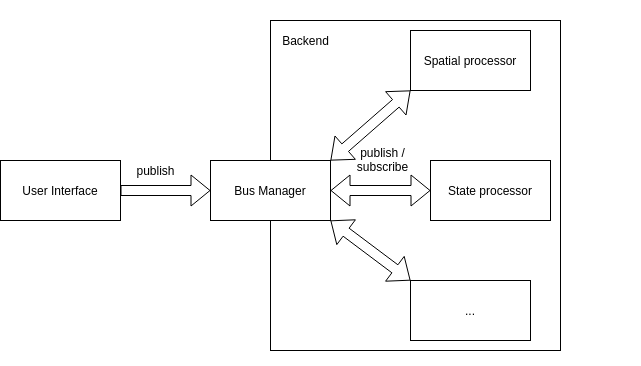
\includegraphics[width=.6\linewidth]{images/couchedit-processors}
  \caption{Publish Subscribe architecture of CouchEdit}
  \label{fig:processors}
\end{figure}

Some of these processors are needed for every type of syntax model, for example the spatial processor, that processes how nodes in the concrete syntax are positioned to each other (above, besides, etc.). Other processors are specific to the given modeling syntax, for example a state chart syntax would require a state processor, that processes if a given graphical object represents a state (usually true if the given node is a rectangle with rounded edges).

A modeling syntax parser for CouchEdit would has to generate these syntax specific processors, while considering multiple design constraints that result from this architecture. Thus a metamodel is needed that can define the desired abstract modeling syntax and specify how a concrete graphical syntax can be mapped to this abstract syntax. While there is ongoing research in the area of relaxed conformance editing and how to link concrete and abstract syntax, it does not immediately become clear what such a metamodel can look like.

\section{Purpose of this Study}
The primary purpose of this study was to develop a metamodel for the CouchEdit framework. This metamodel is supposed to provide a comprehensive and easy to use way for defining new modeling languages. To evaluate the applicability of this metamodel, furthermore a prototypical code generator was implemented, that can comprehend this newly designed metamodel and translate it into a source code implementation.

This extension of the CouchEdit framework is supposed to improve developer accessibility and framework flexibility. While a code generator means that the system still has to be recompiled for every modeling syntax, it still becomes easier to support new modeling syntaxes as the metamodel abstracts away from the actual source code implementation and thus requires less knowledge about the CouchEdit framework.


\section{Research Questions}
\comment{rewrite to fit thesis}

The primary goal of this research will be the development of a metamodel for the CouchEdit framework. This imposes multiple questions which are to be answered in order to design and evaluate the designated metamodel.

\begin{description}
  \item[RQ1:] Is it possible to define a concise metamodel that covers CouchEdits complete feature set?

        If this is not possible, the following question has to be answered.
        \begin{description}
          \item[RQ1.1:] How could the feature set be narrowed down, without impacting the frameworks capabilities too much?
        \end{description}

  \item[RQ2:] What requirements does the CouchEdit architecture impose onto a metamodel?

        The architectures characteristics and quirks have to be considered when designing the language. For example, the publish and subscribe pattern, could make it easy to introduce nonterminating processing chains, which the metamodel should prevent where possible.

  \item[RQ3:] How applicable is the designed metamodel for defining new modeling syntaxes?

        \begin{description}
          \item[RQ3.1] Is it possible to express common modeling syntax concepts in a clear and concise way?
          \item[RQ3.2] Are complex concepts still expressible without causing to much convolution?
        \end{description}
\end{description}


\section{Methodology}
\comment{also only pasted right now}

As this research strives to develop a new metamodel suitable for the CouchEdit framework, it will be conducted in accordance to the Design Science Research (DSR) approach. According to V. Vaishnavi et al. a design science research process consists of five steps \cite{Vaishnavi2004}.

\subsection{Problem Awareness}
The first step of a design science research is the identification of existing problems. As specified in section \ref{sec:problem_statement}, it was identified that the current CouchEdit implementation lacks an user friendly way of adapting it to different modeling syntaxes and that it is unclear how a metamodel for this architecture would look like.

\subsection{Suggestion}
With a clear definition of the problem, objectives can be proposed which have to be achieved in order to solve this problem. The first objective of this research is to develop a metamodel for the CouchEdit architecture. To be more precise, a metamodel is to be designed, that can be used to specify model syntax definitions which map concrete graphical syntaxes to Abstract syntax models and is applicable to CouchEdit's architecture. The second objective is to implement a prototype that provides proof of concept for the applicability of the design metamodel.


\subsection{Development}
The primary goal of a design science research is the development of artifacts.
The first artifact to be developed in this research will be a metamodel, that can be used to define new modeling syntaxes for a relaxed conformance editor and is applicable to CouchEdit's architecture. The second artifact that is to be developed, is a prototypical code generator that can translate the developed metamodel into a CouchEdit implementation which will be able to process the defined modeling syntax.

To this end, the first sub step of the development stage will be to do a comprehensive analysis of CouchEdits architecture. In his work L. Nachreiner describes in detail, which modeling features the framework covers and how they are implemented \cite{nachreiner_couchedit_2020}. For each of these features, a sub metamodel has to be designed that can be used to define the given feature (RQ1). The approaches of \cite{minas_specifying_2001} and \cite{fondement_making_2005} provide a DSL implementation from which concepts for potential metamodels could be derived. If for one of the features, a suitable metamodel cannot be found, it would have to be evaluated if the feature could be simplified or even dropped (R1.1). After designing sub metamodels for all features, they then have to be composed together, which results in a first version of an applicable metamodel. 

in the next sub step, the code generator will be implemented, this is an iterative step. first, an implementation will be developed on the basis of the designed metamodel, this should reveal further requirements imposed by CouchEdits architecture (RQ2). The metamodel then has to be adjusted to account for these requirements, which in turn requires changes of the implementation until no further requirements can be deduced. Because of time constraints it will not be possible to implement all of the metamodel's features, instead the prototype will cover a minimal feature set that still suffices to demonstrate the metamodel's applicability for selected modeling syntaxes.

\subsection{Evaluation}
Now that the desired artifacts are fully developed it has to be evaluated how well they do their designated task. The metamodel as the primary artifact of this research has to be evaluated in terms of its applicability to its designated domain. To this end, the metamodel will be demonstrated on the basis of different modeling syntaxes, this should highlight areas in which the metamodel's design excels, as well as design flaws and limitations (RQ3). If time allows, potential flaws can be addressed by returning back to the development phase and revising the artifacts, otherwise flaws are to be highlighted so that future works can address them.

\subsection{Conclusion}
The conclusion stage marks the end of a DSR and the results are written up. This works written part will be the resulting bachelor's thesis as well as all source code and documentation.


\section{Limitations}
\comment{\dots}
\begin{itemize}
  \item not a complete metamodel designed. common language concepts ignored
\end{itemize}

\section{Thesis Structure}
\comment{\dots}
\chapter{Related Work and Fundamentals}

this chapter lays out a knowledge foundation, required in later sections \comment{(*barf* horribly written)}. First an extensive introduction into the CouchEdit architecture is given, that will be needed later on to understand design decisions. Following that, the syntax of the petri net and statechart modeling languages are introduced, which are used in Chapter \ref{chap:design} to explain concepts of the proposed metamodel. Finally, related work is being explored \comment{(to short)}. 


\section{Methodology}
\comment{also only pasted right now}

As this research strives to develop a new metamodel suitable for the CouchEdit framework, it will be conducted in accordance to the Design Science Research (DSR) approach. According to V. Vaishnavi et al. a design science research process consists of five steps \cite{vaishnavi_design_2004}.

\subsection{Problem Awareness}
The first step of a design science research is the identification of existing problems. As specified in section \ref{sec:problem_statement}, it was identified that the current CouchEdit implementation lacks an user friendly way of adapting it to different modeling syntaxes and that it is unclear how a metamodel for this architecture would look like.

\subsection{Suggestion}
With a clear definition of the problem, objectives can be proposed which have to be achieved in order to solve this problem. The first objective of this research is to develop a metamodel for the CouchEdit architecture. To be more precise, a metamodel is to be designed, that can be used to specify model syntax definitions which map concrete graphical syntaxes to Abstract syntax models and is applicable to CouchEdit's architecture. The second objective is to implement a prototype that provides proof of concept for the applicability of the design metamodel.


\subsection{Development}
The primary goal of a design science research is the development of artifacts.
The first artifact to be developed in this research will be a metamodel, that can be used to define new modeling syntaxes for a relaxed conformance editor and is applicable to CouchEdit's architecture. The second artifact that is to be developed, is a prototypical code generator that can translate the developed metamodel into a CouchEdit implementation which will be able to process the defined modeling syntax.

To this end, the first sub step of the development stage will be to do a comprehensive analysis of CouchEdits architecture. In his work L. Nachreiner describes in detail, which modeling features the framework covers and how they are implemented \cite{nachreiner_couchedit_2020}. For each of these features, a sub metamodel has to be designed that can be used to define the given feature (RQ1). The approaches of \cite{minas_specifying_2001} and \cite{fondement_making_2005} provide a DSL implementation from which concepts for potential metamodels could be derived. If for one of the features, a suitable metamodel cannot be found, it would have to be evaluated if the feature could be simplified or even dropped (R1.1). After designing sub metamodels for all features, they then have to be composed together, which results in a first version of an applicable metamodel. 

in the next sub step, the code generator will be implemented, this is an iterative step. first, an implementation will be developed on the basis of the designed metamodel, this should reveal further requirements imposed by CouchEdits architecture (RQ2). The metamodel then has to be adjusted to account for these requirements, which in turn requires changes of the implementation until no further requirements can be deduced. Because of time constraints it will not be possible to implement all of the metamodel's features, instead the prototype will cover a minimal feature set that still suffices to demonstrate the metamodel's applicability for selected modeling syntaxes.

\subsection{Evaluation}
Now that the desired artifacts are fully developed it has to be evaluated how well they do their designated task. The metamodel as the primary artifact of this research has to be evaluated in terms of its applicability to its designated domain. To this end, the metamodel will be demonstrated on the basis of different modeling syntaxes, this should highlight areas in which the metamodel's design excels, as well as design flaws and limitations (RQ3). If time allows, potential flaws can be addressed by returning back to the development phase and revising the artifacts, otherwise flaws are to be highlighted so that future works can address them.

\subsection{Conclusion}
The conclusion stage marks the end of a DSR and the results are written up. This works written part will be the resulting bachelor's thesis as well as all source code and documentation.


\section{CouchEdit}
\label{sec:CouchEdit}
As noted in section \ref{sec:problem_statement}, the CouchEdit framework is based on the Ideas of Van Tendeloo, et al. \cite{van_tendeloo_concrete_2017}. In their paper, the authors criticize that classic approaches to modeling frontends usually create one monolithic construct, which handles both the graphical model display as well as the corresponding abstract syntax. This creates tight coupling between the two, which causes low flexibility of the UI and requires high effort, if new features are to be implemented. 

They propose to solve this, by defining two metamodels, one describing the graphical syntax and one the abstract syntax. The render syntax metamodel specifies graphic primitives that are needed to compose a given modeling syntax. instances of this metamodel are managed by the frontend and a user can manipulate this concrete syntax directly by adding, deleting or modifying Elements in the UI (if the frontend allows changes). On The other side stands the abstract syntax metamodel, it describes the conceptual representation of a modeling syntax. Instances of this metamodel are managed by the backend. To then connect these two metamodels, a further metamodel, called concrete syntax metamodel, can be defined. This concrete syntax metamodel specifies transformations to translate concrete representation into an abstract model and backwards (Figure \ref{fig:transmm}). 

\begin{figure}
  \centering
  \includegraphics[width=.7\linewidth]{images/"presentation - transfere-metamodel"}
  \caption{Depiction of CouchEdit's approach to separating graphical and abstract representation}
  \label{fig:transmm}
  \end{figure}

Following this architecture, CouchEdit separates frontend from the abstract syntax model. The frontend at its core is a simple vector drawing application, that implements further functionality for diagrams. The backend is then analyzing these vector graphics and translating it into a corresponding abstract syntax. For this, the backend utilizes a set of independent components, that each are responsible for detecting different aspects of the diagram. Each Component contains its own state, when a component detects changes and updates its state, it also publishes these changes so that other components, interested in these changes, can use them.  

This architecture, has the advantage of being very detangled. this allows for components to be improved in isolation from the rest of the system and the clear separation of concerns makes it easier to understand, which component is responsible for what task. Furthermore, components can be swapped out depending on what syntax transformations are needed for the configured modeling syntax.



\subsection{Data Model}
CouchEdit uses a Hypergraph of Elements and Relations to represent its data. Each component has its own instance of this graph that only contains the area of the graph, that is interesting to this component. A component can manipulate its personal graph and make these changes known to the system, so that other components can manipulate their personal graph.


\subsubsection{Elements}
Elements are the base type of CouchEdits hypergraph. Every type of node in this graph inherits from the Element type. As all hypergraph instances should be independent from each other, it is not possible to access Elements via their object reference, thus every Element has an unique id, that kann be used to reliably identify an Element across multiple graphs. Elements also have a probability attribute, that denotes how probable it is that this Element is the result of a correct interpretation of the given Hypergraph. This probability object can be set to Explicit, which means that, either this Element describes a factual truth or it was set by the User. Furthermore, an Element subtypes can introduce further attributes, that contain important information for the given type.

\subsubsection{Relations}
Relations represent Edges of the Hypergraph. Each Relation connects a set of source Elements to a set of target Elements. They also inherit from the Element type and thus can recursively be connected with relations themselves. The connected vertices are referenced using the ElementReference class. This class holds an Elements unique id as well as its type, which then can be used to find a referenced Element in the hypergraph. Figure \ref{fig:relations} shows the implementation of Relations. 

\begin{figure}[ht]
  \centering
  \includegraphics[width=.8\linewidth]{images/"csd - relation"}
  \caption{Class diagram of Relations}
  \label{fig:relations}
\end{figure}

Via subtyping of relations, it is possible to have multiple different relations between the same two elements, that all describe different kinds of connections. While Relations can connect sets of source and target vertices, the most common relation sub type is the OneToOneRelation, it describes a connection between exactly one source and one target Element. 


\subsubsection{Graphic Objects}
graphic objects represent atomic elements, that the user interacts with, via the Frontend. An important decision, when designing an Editor is the question on how granular singular graphic objects should be. 

On a basic level, graphic objects can consists of either pixels or vectors. a pixel based Approach would require a visual recognition preprocessor, that composes the state of pixels in to comprehensible graphic primitives. While such form of image recognition is outside the scope of the CouchEdit project, similar projects such as FlexiSketch \cite{wuest_flexisketch_2015} show the possibilities this approach enables.

Most modeling approaches with some form of abstract syntax processing capabilities, build graphic elements with the purpose of representing a specific element of the abstract syntax. As a result these graphic elements are very strict in their graphical representation. 

CouchEdit Follows the Classification of Costagliola, et al. \cite{costagliola_classification_2002}. This classification defines a graphic element on its lowest level as a primitive graphic shape (e.g circle, line) \comment{(read up if thats actually what costagliola are doing)}. Via sub-classing, a single graphic object can increase in complexity. Such complex graphic object can have  



\begin{itemize}
  \item attribute bag
\end{itemize}


\subsection{Processors}
In CouchEdit the mentioned independent components, are represented as 
subscribe to element types, publish new diffs, connected to bus, model diffs

\subsubsection{Core Processors}
\begin{itemize}
  \item Spatial Abstractor 
  \item ConnectionEnd Processor
\end{itemize}

\subsection{Services}



\begin{itemize}
  \item renderMM - ConcreteMM - AbstractMM
  \item publish/subscribe pattern
  \item attribute bags
  \item model repository
  \item suggestions
\end{itemize}

\section{Modeling Languages}

\comment{\dots}

% \subsection{Graphical Language Theory}
\subsection{Petri Nets Syntax}
In the following, design considerations are explained using a simple petri net syntax. Figure \ref{fig:petrinets_metamodel} shows the abstract syntax metamodel of the used Petri nets syntax. The Petri nets conceptual representation consists of places and transitions. Places also have a token count. each place can have a variable amount of incoming and outgoing transitions, while transitions can have any amount of incoming and outgoing places. 

\begin{figure}[H]
  \centering
  \includegraphics[width=.7\linewidth]{images/"csd - petrinet-metamodel"}
  \caption{Metamodel for a simple petri net abstract syntax}
  \label{fig:petrinets_metamodel}
\end{figure}

The graphic representation of Petri nets is described in table \ref{tab:petri-primitives}. Places are usually represented as circles, while Transitions are depicted as slender rectangles. The number of small black circles inside a place represent this places token count. Furthermore places and transitions possess a label close to their bounding box, that determines their name. Lastly places and transitions have directed connection lines between then. Each connection points from a place or transition towards an element of the opposite type and represents man outgoing connection for the source element and an incoming connection for the target element. A simple concrete instantiation and its corresponding abstract representation is shown in figure \ref{fig:petrinets_example}.

\begin{table}[ht]
  \centering
\begin{tabular}[width=.1\linewidth]{| Sc | Sc | Sc | Sc | Sc |}
  \hline
  Place & Transition & Token & Label & Connection 
  \\
  \hline
  \includegraphics[width=.1\linewidth]{images/"petrinet - place"} 
  & 
  \includegraphics[width=.1\linewidth]{images/"petrinet - transition"} 
  & 
  \includegraphics[width=.1\linewidth]{images/"petrinet - token"}
  & 
  \includegraphics[width=.1\linewidth]{images/"petrinet - label"}
  & 
  \includegraphics[width=.1\linewidth]{images/"petrinet - connection"} 
  \\
  \hline
\end{tabular}
\caption{graphic primitives used to describe petri nets}
\label{tab:petri-primitives}
\end{table}

\begin{figure}[ht!]
  \centering
  \begin{subfigure}[t]{.4\textwidth}
    \centering
    \includegraphics[width=.9\linewidth]{images/"petrinet - example"}
    \caption{concrete syntax}
    \label{subfig:petriconcrete}    
  \end{subfigure}
  \begin{subfigure}[t]{.45\textwidth}
    \centering
    \includegraphics[width=\linewidth]{images/"csd - petrinet-example"}
    \caption{abstract syntax}
    \label{subfig:petriabstract}    
  \end{subfigure}
  \caption{concrete and abstract representation for a simple Petri net example}
  \label{fig:petrinets_example}
\end{figure} 

\subsection{Statechart Syntax}


\begin{figure}
\centering
\includegraphics[width=.7\linewidth]{images/"csd - new-statechart-metamodel"}
\caption{Abstract Metamodel of State charts}
\label{fig:statechartmm}
\end{figure}





\comment{...}
\chapter{Related Work}
\label{chap:related_work}
There are multiple projects that implement a form of relaxed conformance editing. But only few of these projects actually define languages that can be utilized to configure different modeling syntaxes. 


\begin{itemize}
  \item TGG
  \item QVT
  \item left side always harder, thus normal TGGS not applicable
\end{itemize}



\comment{we need some more related work. probably talk a bit about TGGs}


\section{Making Metamodels Aware of Concrete Syntax}
\label{sec:fondement}
in their work, Making Metamodels Aware of Concrete Syntax \cite{fondement_making_2005}, F. Fondement and T. Baar argue that, while abstract syntax definitions are standardized, most language specifications keep the concrete syntax informal. To solve this problem, they propose an approach to defining the concrete syntax and how to link it to the abstract representation.

For this, the authors complement every class of the abstract syntax with a corresponding display scheme. This display scheme is compose of two parts, an iconic and a constraining part. The iconic part defines a set of \texttt{DisplayClasses}, these \texttt{DisplayClasses} group Graphical Objects together into visual representation object. On the other hand, the constraining part links these \texttt{DisplayClasses} to an abstract syntax element. This link is realized using \texttt{DisplayManagers}. A \texttt{DisplayManager} serves as connection between exactly one model element of the abstract syntax and one display object and has the task of syncing the abstract to the concrete representation. An example of this architecture is depicted in figure \ref{fig:fondement_dm}, for a Petrinet place element. The graphical primitives, a place is composed of, are mapped to a place \texttt{DisplayClass}, to build a places iconic part. This iconic representation is then attached to a place model element, using a place \texttt{DisplayManager}.


\begin{figure}[H]
  \centering
  \includegraphics[width=\linewidth]{images/"csd - fondement-example"}
  \caption{Example representation of a Petrinet place element}
  \label{fig:fondement_dm}
\end{figure}

A DisplayManager has to keep abstract and concrete representation in sync, for this Fondement and Baar utilize OCL invariants, which are defined on the DisplayerManager. For example, an invariant to sync the name of place display schemes could look as following:

\begin{lstlisting}[language=OCL,captionpos=b,caption={OCL Invariant that syncs the name attribute of \texttt{DisplayClass} and model element.}]
context PlaceDM
inv: self.me.name->exists() implies
        self.me.name = self.vo.name.text
\end{lstlisting}

The Authors keep open, how the mapping from graphical primitives to a display object could be implemented. while the metamodel proposed in this thesis does not introduce an extra layer of abstraction in form of these \texttt{DisplayClasses}, it still is inspired heavily by Fondement's and Baar's work. Especially the constraining part that utilizes \texttt{DisplayManagers} to sync abstract and concrete syntax, served as primary inspiration for the proposed architecture.

In the work "Correctly defined concrete syntax" \cite{baar_correctly_2008}, Baar furthermore provides an algorithm to check syntactic correctness of the concrete representation. While checking the concrete syntax for correctness is out of scope of this work, a future implementation would have to provide the user with syntax checking capabilities, to make sure that the model, designed in the editor is syntactically correct.


\subsection{DiaGen/DiaMeta}
DiaGen is 

\chapter{Design Concept}
% \raggedbottom
\label{chap:design}
In Section \ref{sec:CouchEdit} it was established that CouchEdit is composed of three distinct metamodels as depicted in Figure \ref{fig:transmm}. Thus is seems apparent that the proposed concept should also be composed of these three metamodels. The definition of abstract syntax metamodels has already standardized approaches (e.g. Ecore\footnote{\url{https://www.eclipse.org/modeling/emf/}}) and thus is mostly ignored. Furthermore, the proposed design currently only supports a render metamodel definition composed of graphic primitives. Complex graphic structures would have to be explored in follow up works. This work focuses on the concrete syntax metamodel, that connects render and abstract syntax and proposes an approach to formalize this connection.

The primary goal of the proposed design is to hide CouchEdit's complexity behind more accessible metamodel definitions. To this end, multiple concepts are employed, that either abstract away from CouchEdit's implementation details, or introduce ways to streamline the translation from concrete to abstract representation. Most of these concepts introduce performance overhead, but as this work focuses on the design aspect, performance analysis and optimization is subsidiary and subject to further research.



\comment{how}
A triple graph grammar is composed of three distinct metamodels, thus the root definition of the CouchEdit configuration is composed of tree distinct areas, as can be seen in figure \ref{fig:metamodel-base}. throughout the chapter, this root model is gradually being extended with new concepts, until finally all utilized concepts have been introduced (complete metamodel is depicted in \ref{fig:complete-metamodel}).

\begin{figure}
  \centering
  \includegraphics[width=.7\linewidth]{images/"csd - metamodel-base"}
  \caption{Composition of the CouchEditConfiguration metamodel}
  \label{fig:metamodel-base}
\end{figure}

\section{Render Metamodel}
CouchEdit's render syntax is realized as a set of graphic objects. The framework in its current form primarily focuses on primitive graphic objects, with its class structure being derived \cite[p.39]{nachreiner_couchedit_2020} from Bottoni and Grau's work, "A Suite of Metamodels as a Basis for a Classification of Visual Languages" \cite{bottoni_suite_2004}. While the notion of complex graphic objects has been introduced in CouchEdit's formal definition, the concept for now only exists in theory. This thesis, because of time constraints, does not explore definition of the concrete syntax all to much and instead focuses only on graphic primitives. The employed render syntax metamodel is describe in figure \ref{fig:concretesyntax}. As shown, it facilitates a basic structure to define graphic primitives needed for the described visual language. Future works would have to explore, how graphic objects could be customized, by integrating attribute bag definitions as well as complex graphic object definitions, to create custom symbols, better suited for certain modeling languages.

\begin{figure}
\centering
\includegraphics[width=.5\linewidth]{images/"csd - rendersyntax"}
\caption{Concrete syntax metamodel used in this thesis}
\label{fig:concretesyntax}
\end{figure}


\section{Abstract Syntax}
\label{sec:abstract-syntax}
As noted before, the abstract syntax can be defined using existing standards. Nonetheless, the translation metamodel needs to reference the abstract syntax at certain points in this chapter. Therefore, a barebones implementation that is derived from Ecore's own metamodel\footnote{\url{https://download.eclipse.org/modeling/emf/emf/javadoc/2.9.0/org/eclipse/emf/ecore/package-summary.html}} definition is defined here (Figure \ref{fig:csd-abstractsyntax}). Notable concepts needed in the definition of an abstract syntax, are foremost definition of classes. This includes, definition of class attributes, as well as concepts such as inheritance and references to other classes. Furthermore definition of simple data types as well as enums is required. \comment{(maybe find source that lists requirements for an abstract syntax metamodel to support what ive written here)} 

\begin{figure}
\centering
\includegraphics[width=.7\linewidth]{images/"csd - abstractsyntax"}
\caption{Used subset implementation of Ecore}
\label{fig:csd-abstractsyntax}
\end{figure}


\section{Language Concepts}
the abstract syntax tree usually differs between programing languages \comment{(another statement i should maybe cite?)}. Therefore, when looking at lower level concepts, found in most programming languages (e.g.: arithmetic, branching), their metamodel representation varies, while the functionality stays the same. For this reason and because there is already enough documentation on how to specify abstract syntax trees, common language concepts will not be defined, as this depends on the actual language implementation. Instead at points where these language concepts would reside, it is only defined what the given metamodel expects from the implementation and example code snippets are given in an unspecified pseudo language. Despite this, there are certain concepts special to the CouchEdit metamodel, which a language implementation would have to realize. these concepts are presented in the following subsections.


\subsection{Helper Functions}
When defining a translation metamodel, it may become useful to relocate certain procedures or algorithms into separate functions. Reasons for this may be, to access it from multiple points in the definition, to implement a recursive structure or, simply to split up complex parts. Thus the metamodel should provide a facility for the definition of custom functions. That being said, the actual metamodel definition is kept ambiguous, as details depend on the given implementation. In the architecture described here, these helper functions are defined on the highest level of the metamodel and thus are available in all statement blocks, but it would also be feasible to move function definitions into sub scopes, should that provide advantages for certain implementations. 

\subsection{Graph Navigation}
\label{sec:abstraction}
Something used a lot in the proposed architecture, is traversal through the hypergraph. It should be possible for the user, to easily get nodes that are adjacent to any given node. In CouchEdit's architecture, this is handled by separate services. This means, that the syntax for reaching a node related by a certain relation type looks something like this: 

\begin{lstlisting}[language=customLang, caption={Example on how to get all GOs contained by a given element \texttt{go}, in the CouchEdit architecture}, captionpos=b]
val containedGOs = relationService
      .getAllElementsRelatedFrom(go, Contains) 
\end{lstlisting} 

The \texttt{getAllElementsRelatedFrom} function, takes a GO and a relation type and returns all GOs that have a relation of the given type, that points from the given GO to themselves. This and similar helper functions are used repeatedly, thus DSL implementations of the here described architecture should provide some form of abstraction to this service call. In the following code snippets, it is assumed that these functions were masked by member function implementations similar to the following:
\begin{lstlisting}[caption={The \texttt{getAllElementsRelatedFrom} function, implemented as a member function eases navigation through the hypergraph}, captionpos=b]
go.getAllElementsRelatedFrom(Contains)
\end{lstlisting}
Implementation in form of such extension functions allows for a more natural navigation trough the hypergraph, which is especially useful when traversing longer distances which will become apparent in the following sections. A list of these navigation functions can be found in Appendix \ref{app:navigationfunctions}.


\section{Syntax Processors}
The primary concern when defining a modeling language with clear separation between concrete and abstract syntax, is the question on how to connect these two distinct models. In this point, the designed architecture draws inspiration from Fondement and Baar \cite{fondement_making_2005}. The author's proposed idea of connecting abstract und concrete syntax, using DisplayManagers, serves as a basis that can be built upon. This approach consists of two parts, recognition and synchronization. 

\subsection{Recognition}
\label{sec:recognition}
The recognition part is concerned with detecting patterns in the graphical syntax that have an abstract syntax representation. For this, Fondement and Baar proposed the introduction of a further abstraction layer. This layer composes the graphic primitives and attributes, which represent a model element, into display classes. But the authors keep possible implementation of this abstraction layer open. Furthermore it did not seem suitable to introduce a further abstraction layer, as most processing in the CouchEdit architecture is applied directly to the concrete syntax hypergraph, thus mapping graphic objects to a new layer would introduce a set of new problems to be solved. Instead the architecture proposed here, tries a different approach. For each type of display manager, a set of constraints can be defined on the hypergraph's graphic objects. Whenever a graphic object satisfies all constraints of a given display manager type it is deemed to be the base element of a concrete representation of this display manager type and an instances of this display manager and corresponding model element are created and connected to the graphic object (Figure \ref{fig:place-recognition}). 

\begin{figure}
  \centering
  \includegraphics[height=8cm]{images/"visualization - place-recognition"}
  \caption{PlaceRecognitionProcessor, adding PlaceDM to a GraphicObject that satisfies constraints}
  \label{fig:place-recognition}
\end{figure}

These constraints can be defined as simple boolean expressions, that each graphic object in the hypergraph, is checked against. The constraints for a place element, could be defined as follows: 

\begin{lstlisting}[language=OCL,caption={Possible constraints to detect GOs representing a place},captionpos=b]
go.shape is Circle
go.allRelatedTo(Contains).isEmpty()
\end{lstlisting} 

These constraints first check if the given GO has the shape of a circle. If that is true, it is also checked if the given GO has any \texttt{Contains} relations pointing toward itself. If that is the case, the given circle is contained by another element and thus not clearly identifiable as a place, as it could also possibly represent a token. A corresponding definition for transitions could look as follows: 

\begin{lstlisting}[captionpos=b,caption={Simple constraint to check for transition representations},label={lst:transition-constraints}]
go.shape is Rectangle
\end{lstlisting}

These are barebones requirements to identify graphical representations and they could be extended by any amount of further constraints to increase the amount of specificity required from the concrete instance.

\subsection{Synchronization}
With the recognition part in place, it is possible to detect graphical representations and attach corresponding abstract instances. Now the synchronization part is responsible to make sure, abstract and concrete representation reflect the same state. To this end, the metamodel allows for the definition of rules on a \texttt{DisplayManager}. This step was explained in detail in \cite{fondement_making_2005}. Fondement and Baar propose the usage of OCL invariants as a language for defining these rules. But as the here defined approach does not implement the display class abstraction layer, the concrete representation has to be queried directly. Furthermore, implementing OCL invariants is not necessary and synchronizations could also be handled by assignment statements, which is done in the following. For a place element there are four aspects that have to be synced:

\begin{enumerate}
  \item Name of the given place
  \item Number of Tokens this place has
  \item Incoming transitions
  \item Outgoing transitions
\end{enumerate} 

Reliably determining a place's name poses some special challenges and requires further concepts, introduced later. Determining the token number, on the other hand is easily implemented using the given tools. A simple rule that syncs this attribute could look something like this:

\begin{lstlisting}[captionpos=b,caption={Rule that syncs the token count of a place element}]
dm.me.tokens = dm.go
                  .allRelatedFrom(Contains)
                  .select(go -> go.shape is Circle)
                  .count()
\end{lstlisting}

This statement ensures that the token attribute of the model element is always equal to the number of all GOs with the shape Circle, that are contained by the base graphic object. In a similar fashion, incoming and outgoing transitions can be defined:
\begin{lstlisting}[captionpos=b,caption={Rule that syncs incoming transitions of a place element},label={lst:incoming-transitions}]
dm.me.incoming = 
      dm.go
          .allRelatedTo(ConnectionEnd,
              rel -> rel.isEndConnection)
          .select(go -> go.shape is Line)
          .collect(go -> go.relatedFrom(ConnectionEnd))
          .select(go -> go.shape is Rectangle)
          .select(go -> go.dm != null)
          .collect(go -> go.dm.me.ref())
\end{lstlisting}

This statement ensures that all transitions, connected to the given DM's GO, by a line, are composed into the list of incoming transitions (Figure \ref{fig:incoming-sync}). This exhibits the usual approach to syncing concrete and abstract representation. 

% Starting from a \texttt{DisplayManager}, the statements query along a path of relations and elements, to determine the correct state of a model element.

\begin{figure}
  \centering
  \includegraphics[height=7.5cm]{images/"visualization - incoming-sync"}
  \caption{A connection line is added to the graph and the PlaceSyncProcessor updates the Place model element}
  \label{fig:incoming-sync}
\end{figure}

\subsection{metamodel}
The resulting sub model for this area of the configuration would look as described in Figure \ref{fig:initial-syntax-model}. The depicted Metamodel allows for the definition of \texttt{DisplayManagers}. A \texttt{DisplayManager} definition, needs a reference model element type from the abstract syntax metamodel. The corresponding DisplayManager can then be inferred from this element. Furthermore, the \texttt{DisplayManager} definition, needs \texttt{Constraints} and \texttt{Rules}. The \texttt{constraints}, are then used by a RecognitionProcessor, to add instances of the inferred \texttt{DisplayManager}. On the other hand \texttt{Rules} are then used by a DisplayManagerProcessor, to keep model elements aligned. As stated, it would be possible to define \texttt{Constraints} and \texttt{Rules} as OCL invariants, similar to what Fondement and Baar did. Another possible implementation would be as statement blocks, where \texttt{Constraints} return boolean values and \texttt{Rules} utilize assignment statements, which would be similar to the here described code snippets. This is not the final iteration of this metamodel as will be shown in the next section.

\begin{figure}
\centering
\includegraphics[width=.7\linewidth]{images/"csd - initial-syntaxprocess-model"}
\caption{First Design of the \texttt{DisplayManager} metamodel}
\label{fig:initial-syntax-model}
\end{figure}


\section{Annotations System}
When assessing the incoming transition rule (Listing \ref{lst:incoming-transitions}), it becomes apparent that checking if the connected GO represents a transition has to be done manually. In the given example, checking if the GO represents a transitions is no big task as transition recognition is handled with only one constraint (Listing \ref{lst:transition-constraints}), but when regarding model elements with multiple constraints, this can become a repetitive and inefficient task. 

To alleviate this problem, the proposed architecture introduces an Annotation system. An Annotation can mark elements of the graph, as satisfying a certain defined pattern. An \texttt{Annotation} is, similar to \texttt{AttributeBags}, a separate element in the graph, that is connected to the element it annotates, with a relation. It has a single value attribute, that indicates its name. Identical to \texttt{DisplayManager} definitions, described in the last section, \texttt{Annotation} definitions take a set of \texttt{Constraints}. Every Element in the graph is then checked against these \texttt{Constraints} and if the Element satisfies all of them, the Annotation is added to the given Element. This behavior is depicted in fig. \ref{fig:kind-recognition} for an example transition \texttt{Annotation}.

\begin{figure}
  \centering
  \includegraphics[height=7.5cm]{images/"visualization - kind-recognition"}
  \caption{\texttt{TransitionAnnotationProcessor} detects a GO that satisfies constraints and adds \texttt{ElementAnnotation}}
  \label{fig:kind-recognition}
\end{figure}

The similarity to the \texttt{DisplayManager} recognition part means that it can actually replace this part, which is done in this concept. Instead of checking \texttt{Constraints} themselves, \texttt{DisplayManager} recognition processors just check if a given GO has a certain annotation attached and if this is true, the corresponding \texttt{DisplayManager} is added. As shown in Figure \ref{fig:Transition-Kind-Recognition}, when a GO, representing a transition is added, the \texttt{TransitionAnnotationProcessor}, first adds an \texttt{ElementAnnotation} with the value \texttt{Transition}. The \texttt{TransitionRecognitionProcessor} then finds the GO which now is annotated with the value \texttt{Transition} and adds a \texttt{TransitionDM}.

\begin{figure}[ht]
\centering
\includegraphics[height=11cm]{images/"visualization - Transition-Kind-Recognition"}
\caption{\texttt{TransitionRecognitionProcessor} adds DM after the \texttt{TransitionAnnotationProcessor} has added a transition \texttt{Annotation}}
\label{fig:Transition-Kind-Recognition}
\end{figure}

With the definition of a convenience member function that checks if an element has a given Annotation, the place incoming transition rule can now be rewritten as follows: 
\begin{lstlisting}[captionpos=b,caption={Improved incoming transition \texttt{Rule}, that also filters for elements with a \texttt{Transition} annotation}]
dm.me.incoming = 
    dm.go
        .allRelatedTo(ConnectionEnd,
            rel -> rel.isEndConnection)
        .select(go -> go.shape is Line)
        .collect(go -> go.relatedFrom(ConnectionEnd))
        .select(go -> go.hasAnnotation(Transition))
        .collect(go -> go.dm.me.ref())
\end{lstlisting}


It is important to note that the \texttt{Annotation} system isn't exclusive to GOs that have an abstract representation. For GO's with a corresponding \texttt{DisplayManager}, the \texttt{DM} type can just be checked to find out if it connects a model elements of a certain type. Rather, the \texttt{Annotation} system can also be used to recognize all sorts of patterns in the graph, that would otherwise have to be checked repeatedly. For example. it could be used to define a stricter check, on what element in a Petrinet Graph represents a token.

\subsection{Metamodel}
As mentioned in the last section, because of the introduction of the \texttt{Annotation} system, the \texttt{DisplayManager} definition model has to be revised. Instead of possessing a set of constraints, \texttt{DisplayManager} definitions, they have a reference to an \texttt{ElementAnnotation} (Figure \ref{fig:revised-syntax-model}).

\begin{figure}
\centering
\includegraphics[width=.75\linewidth]{images/"csd - revised-syntaxprocess-model"}
\caption{Revised SyntaxProcessor metamodel that now includes the kind system}
\label{fig:revised-syntax-model}
\end{figure}


\section{Plugins}
\label{sec:plugins}

While the invariant for incoming transitions, is sufficient for an initial example, it has two mayor flaws. Firstly, it is not checking if the connecting line has an arrow end and secondly only lines that are drawn from the transition towards the Place, are treated as incoming lines, which is defined by the isEndConnection attribute of the ConnectionEnd relation. Fixing these issues in form of an invariant would be to verbose for such a common pattern.

For this reason, a Plugin system is introduced. Plugins are predefined Processors that process specific parts of the hypergraph. These processing areas are not as integral as the ones solved by the core processors and thus are opt-in. Furthermore certain plugin processors can be configured which allows them to cover a wider field of use cases. One example of such a plugin would be the TransitionProcessor. It looks for line GraphicObjects and checks if they connect two other GOs. If that's the case, the processor adds either a TransitionTo relation or a TransitionBetween relation (fig. \ref{fig:transition-plugin}), depending on if the line's arrow ends indicate a directed or undirected transition. Adding this Plugin allows for a final rewrite of the incoming transitions statement:

\begin{lstlisting}[language=OCL]
dm.me.incoming = 
    dm.go
        .allRelatedTo(TransitionTo)
        .select(go -> go.hasKind(Transition))
        .collect(go -> go.dm.me.ref())
\end{lstlisting}

\begin{figure}[ht]
\centering
\includegraphics[height=7.5cm]{images/"visualization - transition-plugin"}
\caption{TransitionProcessors adds TransitionTo relation on detecting a directed line}
\label{fig:transition-plugin}
\end{figure}



\subsection{Label Processor}

Defining a transformation to sync a place's name has been postponed until now, because it poses multiple new challenges. When determining, if a label represents the name of a place object, multiple aspects have to be minded. 
\begin{enumerate}
  \item How close is the label to the place.
  \item Are different graphic objects in the vicinity that could be associated with this label.
  \item Are there other labels that could represent the name of this place.
\end{enumerate}

While possible, checking all these conditions in a syncing statement would require several dozen lines of code and cause a lot of overhead, as for every place, whenever syncing its state, the relation possibility, to all Labels and per transitivity, their possible relation to a different element, has to be calculated. Thus, the idea of building a plugin that handles these calculations arises.

The basic idea of the LabelProcessor is, to add LabelFor relations from labels to other graphic objects, and to utilize it's probability attribute to describe how probable it is, that the label is labeling the given graphic object. To be applicable to multiple concrete syntaxes, this plugin poses a new set of requirements: 
\begin{enumerate}
  \item Modeling syntaxes require different spatial relations between label and graphic object (label can be contained, surrounding, above/below, etc.).
  \item Different GO shapes require different algorithms to calculate the probability (proximity to a circle cant be calculated the same way as proximity to a rectangle is)
  % \item multiple LabelFor relations from a single Label should be able to influence the probability of these relations.
  \item If a graphic object needs a label relation, depends on its kind. For example, while tokens have the same shape as places, only places can have a labels and giving tokens a label relation would needlessly increase ambiguity.
  \item Some label relations can take precedence over others. For example, when considering Statecharts, a label that is contained by a simple state, can't describe a transition trigger event.
\end{enumerate}

\subsubsection{Label Sub Processor}
The LabelProcessor, implements a set of sub processors. Each sub processor is responsible for calculating LabelFor relations for a different type of spatial relation between label and  graphic object of a certain shape. For example, the CircleOuterLabel sub processor calculates the LabelFor relation between a circular shaped graphic object and a surrounding label. This means, for every combination of primitive shape and spatial relation, a different sub processor is needed. Each sub processor takes an element kind and a label. It then finds all graphic objects with its designated shape type and filters them by the given element kind. The resulting GOs then receive a LabelFor relation from the given label, with a probability calculated by an algorithm implemented in the sub processor. 

\subsubsection{Label ProcessingChain}
When regarding requirement 4 it becomes clear that simply enabling the sub processors, that are needed for a given modeling syntax, isn't enough. A mechanism is needed that allows for different sub processor configurations to influence each other. Therefore the concept of a ProcessorChain was introduced (fig. \ref{fig:labelprocessor-config}). A ProcessorChain allows for the configuration of sub processors by introducing an arithmetic like operation system. ProcessorChains can either be Operations or Terminals. Terminals represent either a sub processor or Nothing. An Operation on the other hand defines a link between two ProcessorChains. Operations possess an Operator that defines how the results of the left hand processing chain should affect the results of the right one. For example, the `and` Operator defines that both processing chains are calculated normally. On the other hand, the `ifEmpty` Operator only calculates the right ProcessorChain, if the left has returned no values. The `ifAmbiguous` Operator ignores the left chain if more than one relation is returned and instead calculates the right side. Using this ProcessorChain, the label processing for Petrinets could be configured as following: 
\begin{lstlisting}
(CircleOuterLabel(Place) and 
RectangleOuterLabel(Transition)) ifAmbiguous Nothing
\end{lstlisting}
This causes the LabelProcessor to calculate outer proximity LabelFor relations for all circular GOs with kind Place and rectangular GOs with kind Transition. should this calculation return more than one possible relation for a given label, the relations are ignored and nothing is returned instead.

\begin{figure}[ht]
\centering
\includegraphics[width=\linewidth]{images/"csd - labelprocessor"}
\caption{Class diagram describing the LabelProcessor's configuration metamodel}
\label{fig:labelprocessor-config}
\end{figure}

This LabelProcessor plugin is by no means a perfect implementation of the given problem, rather it gives a general idea of the purpose and applicability for the plugin system, as well as an idea of how specialized the definition of plugin configurations can become. The requirements of plugin configurations, forces DSL implementations of this metamodel to potentially be updated every time a new plugin with custom configuration is added to the system. Alternatively an approach for more general plugin configuration has to be explored


In this chapter, the developed metamodel was introduced step by step. The base idea for this metamodel was derived from Fondement and Baar \cite{fondement_making_2005}, but was partially modified and extended to serve requirements posed by the CouchEdit architecture. The complete metamodel is depicted in Figure \ref{fig:complete-metamodel}. 
\chapter{Prototype}
\label{ch:prototype}
Along side the development of the metamodel, described in \Cref{ch:design}, a prototype was developed as well, which serves as a proof of concepts for design decisions made. This prototype is realized as an extensions of \textsc{CouchEdit}'s current existing prototype, developed by Nachreiner and presented in \cite{nachreiner_couchedit_2020}.

\textsc{CouchEdit}'s current running prototype is completely written in Kotlin\footnote{\url{https://kotlinlang.org/}}, a programing language with the ability to compile to the Java virtual machine platform. Thus, Kotlin enables access to Java's ecosystem of libraries and Frameworks. TornadoFX\footnote{\url{https://tornadofx.io/}}, a JavaFX wrapper, is used as UI Framework. As a modeling tool, GEF\footnote{\url{https://www.eclipse.org/gef/}} was integrated. Dependencies are handled using the dependency injection framework Guice\footnote{\url{https://github.com/google/guice}}, which integrates perfectly with \textsc{CouchEdit}'s modular architecture. Detailed information about the current prototype and its features are presented in \cite{nachreiner_couchedit_2020}.

In theory, integrating \textsc{CouchEdit} with a parser that can evaluate language configurations at runtime would be preferable. This would make it possible to hot swap configurations while the software is running. Instead, the prototype was extended by a code generator. This has multiple reasons. The current implementation is relying on the existence of class definitions. Meaning, at certain points in the code object types are checked. A runtime parser would have to either create workarounds for these type checks or compile the needed classes at runtime, using byte code manipulation. A code generator can generate all class definitions directly and thus solves this problem without any extra effort. Furthermore a code generator can work with a metamodel that is not fully defined. As noted in \Cref{ch:design}, low level languages concepts were not fully defined, as they depend on the actual language implementation. To circumvent the problem of having to define an actual language implementation for these low level concepts, the implemented parser opts to simply replace these parts with strings. Statements and expressions, can simply be written directly into these Strings, which are then placed into the generated code, without any further analysis of their correctness. This means, that these strings have to contain Kotlin code. Furthermore, needed language concepts (\Cref{sec:language-concepts}) have to be provided by the Kotlin implementation itself.

The code generator was implemented as a separate sub module of the existing prototype. It contains its own runnable method that, when executed, will generate a new module. This module provides the language configuration, which is loaded by the model application when started and automatically configures the application for this modeling syntax. For code generation purposes FreeMarker\footnote{\url{https://freemarker.apache.org/}} is used. FreeMarker is a language agnostic template engine, and therefore allows for the generation of kotlin code out of the box.

To ease the effort of defining language configurations, it was also decided to implement an internal DSL, using Kotlin's integrated capabilities\footnote{\url{https://kotlinlang.org/docs/reference/type-safe-builders.html}}. Furthermore, Kotlin's script API was utilized, which allows for the relocation of configurations into script files. These files then can be loaded at runtime.

\section{Kotlin DSL}
The \textsc{CouchEdit} DSL is composed of three distinct parts, each representing one of the sub metamodels defined by the \texttt{\textsc{CouchEdit}Configuration}. Each \textsc{CouchEdit} configuration consists of three files, \texttt{RenderMM}, \texttt{ConcreteMM} and \texttt{AbstractMM}, describing each of the three sub metamodels, the \textsc{CouchEdit} configuration is composed of.

\subsection{Render DSL}
Given the simplicity of the \texttt{RenderMetamodel} defined in this work, the corresponding DSL does not encompass much grammar. The RenderMM DSL provides a set of constants, each representing a shape supported by the framework. A configuration takes a set of these constants. Future work would have to look at how graphical attributes work with the system as well as integration of complex graphic objects. An example of such a \texttt{RenderMM} instance for a Petrinets configuration, is shown in \Cref{lst:petri-rendermm}.

\subsection{Abstract DSL}
It was noted in \Cref{sec:abstract-syntax} that the \texttt{AbstractSyntaxMetamodel} can be defined using existing tools such as Ecore. As developing a functioning Ecore parser was deemed to complex, the prototype instead implements a barebones grammar that allows for the definition of a subset of the Ecore metamodel. Notably the DSL allows for the definition of enums and classes. While interface definitions are worthwhile as well, they are not yet supported.

% \textsc{\textbf{Classes:}} Class definitions are used to define classes 

% \lstinputlisting[captionpos=b,caption={Place \texttt{Class} definition},linerange={6-11}]{code/configs/petrinets/AbstractMM.kts}

% \textsc{\textbf{Enums:}}

% \lstinputlisting[captionpos=b,caption={PseudoStateKind \texttt{Enum} definition},linerange={15-19}]{code/configs/statechartsnew/AbstractMM.kts}

\texttt{StructuralFeatures} allow for the definition of attributes a class possesses. Most Notably they allow for the definition of attributes and references to other classes. A \texttt{StructuralFeature} holds a name, as well as upper and lower bound definitions, where an upper bound of `-1` indicates that it is unbound. Furthermore a \texttt{StructuralFeature} can hold a default value. The DSL allows for the definition of \texttt{StructuralFeatures} in form of three symbols, \texttt{attr}, \texttt{ref} and \texttt{comp}. \texttt{attr} is used to define simple attributes, a class definition can hold. Currently supported \texttt{AttributeTypes} are: boolean, string, integer, double, unspecified Java classes and objects, as well as any enums defined. \texttt{ref} and \texttt{comp} can be used to define references to other classes. Because of limitations imposed by the Kotlin DSL, enum as well as class reference names have to be wrapped into string literals. While \texttt{ref} defines standard references, \texttt{comp} defines compositions. This plays an important role When generating source code from this configuration. References define connections to objects, that can exist by themselves. In the \textsc{CouchEdit} architecture that means, they have to exist in the applications hypergraph. Thus they can only be referenced, using \texttt{ElementReferences}. On the other hand, composition objects do not exist as separate entities in the graph und therefore must not be referenced using \texttt{ElementReferences}. the \texttt{AbstractMM} definition for Petrinets is shown in \Cref{lst:petri-abstractmm}.

\subsection{Concrete DSL}
The \texttt{ConcreteMM} definition is the centerpiece of the developed artifact, thus defining this part was main focus during the development process. Similarly to the metamodel defined in \Cref{ch:design}, the \texttt{ConcreteMM} DSL is composed of three distinct concepts, with an additional possibility of defining helper functions. Each of the concepts is defined in its own scope.


\textbf{Helpers:} The \texttt{helpers} scope allows for the definition of \texttt{helper} functions. \texttt{helper} definitions take a name, multiple arguments, as well as a body. The functions return value is determined by the bodies last statement, as is done in all following statement blocks. Usually Kotlin can infer the type of this value by itself. In the case a recursive function is implemented, the return type has to be specified as Kotlin will run into recursive type checking problems. Because of the nature of a variable argument count, introduced by \texttt{param} definitions, body and return type have to be specified using Kotlin's named parameter syntax\footnote{\url{https://kotlinlang.org/docs/reference/functions.html\#named-arguments}}. To reduce the overhead of implementing functions, parameters as well as the function body have to be written in string literals. Thus these values can then later be inserted into the generated kotlin source code. This enables access the full Kotlin functionality without having to do any extra work. On the flipside, that means the an IDE can not give any syntax checking for code segments encoded into string literals.

\textbf{Plugins:} The \texttt{plugins} scope allows available plugins to be enabled. Similar to the \texttt{RenderMM} DSL, the plugins scope provides a set of constants, each representing an available plugin. Furthermore, plugins that require additional configuration have their own scope, which provides the grammar required to specify a configuration for this plugin.

\textbf{Patterns:} The \texttt{patterns} scope allows for the definition of new pattern types. Each new pattern type is marked by a \texttt{def} block which contains the patterns name, followed by a new scope. The scope contains all constraints that a \texttt{GO} has to satisfy, to be marked with this pattern. A constraint is by a `+`, followed by a string literal. The string literal represents a complete statement block and thus can contain multiple statements, where the last statement represents the return value. These constraint blocks must return a boolean value und thus, have to always end in a boolean expression. Furthermore the constraints are completely isolated from each other. This means, casting the \texttt{GO} in one constraint will have no effect on following constraints. On the other hand, these constraints are executed in the order they are defined in. If one constraint fails, following constraints will not be checked. this offers the possibility to safely cast a \texttt{GO} in all constraints, when a previous constraint has verified the objects type.

\textbf{DisplayManagers:} The \texttt{displayManagers} scope allows for the definition of new \texttt{DisplayManagers}. Each new manager definition is marked by a \texttt{def} block, that contains a string literal specifying the abstract model element and possibly one literal specifying the corresponding pattern. 
% If no pattern name is given, the definition represents an \texttt{AbstractDisplayManager}. 
Rules are defined in the same way as pattern constraints are. A rules statement block on the other hand has no specific return type. Instead they directly act on a given \texttt{DisplayManager} and manipulate the corresponding model element. Should two different rules manipulate the same attribute, the rule defined last will overwrite changes done by the first one. Rules can be defined in a way as to not change any values of the model element. An Example definition for a Petrinets \texttt{ConcreteMM} configuration is shown in \Cref{lst:petri-concretemm}.

\section{Example Configurations}
\label{sec:example-configs}
This section exhibits two implementation examples, based on the model syntaxes presented in \Cref{sec:modeling-languages}.

\subsection{Petrinets}
\label{sec:petri-impl}
As a first example a Petrinets configuration was implemented. This configuration follows the model defined in \Cref{sec:petrinets}, while the complete implementation is shown in \Cref{app:petri}. The complete configuration script, composed of RenderMM, AbstractMM and ConcreteMM, is \petriConfigLoC lines long\footnote{These metrics were counted with the cloc tool: \url{https://github.com/AlDanial/cloc}}. The Kotlin code generated by this configuration encompasses \petriGeneratedLoC lines. 

Shapes configured in the RenderMM (\Cref{lst:petri-rendermm}) are, circle, rectangle, line and label. With future development of a more sophisticated RenderMM configuration, the circle shape could be defined separately, once as a small black circle and once as a bigger circle without fill color. 

The AbstractMM (\Cref{lst:petri-abstractmm}) definition has two Class definitions. The Place Class has one attribute name of type string, another attribute tokens, with type integer, a fixed bound to "1" and a default value "0". Furthermore the Place Class has two references, incoming and outgoing, with the type Transition and an unlimited upper bound, indicated by "-1". The Transition Class is defined in the same fashion.

The ConcreteMM (\Cref{lst:petri-concretemm}) definition has the connection and label  plugin, mentioned in \Cref{sec:plugins} enabled. The connection plugin in its current iteration does not take a configuration. The label plugin on the other hand is configured to detect labels that surround a graphic object with the pattern Place or Transition. If this results in more than one possible LabelFor relation, the result is discarded as noted by "\texttt{ifAmbiguous nothing}". One \texttt{helper} was defined, which finds the text, a place or transition is labeled with. The \texttt{patterns} scope has three patterns defined, \texttt{PLace}, \texttt{Token} and \texttt{Transition}. \texttt{Place} and \texttt{Transition} constraints are defined similar to the examples given in \Cref{sec:recognition}, but the \texttt{Transition} pattern contains an additional constraint that checks if a rectangle has one side at least double the length of the other side. The \texttt{Token} pattern is used to detect elements that actually represent a token, to ease the process of syncing the token count. The \texttt{DisplayManagers} scope has two definitions, one \texttt{PlaceDM} and one \texttt{TransitionDM}. The \texttt{PlaceDM} connects \texttt{Place} pattern and \texttt{Place} model element.

The Petrinets configuration provides an example on how to use the developed prototype to define \textsc{CouchEdit} configurations. 

\subsection{Statecharts}
\label{sec:state-impl}
as a second example, the Statecharts syntax defined in \Cref{sec:statecharts} was realized. But the configuration does leave out some of the described functionality. This was done to align this implementation closer with the example presented in \cite{nachreiner_couchedit_2020}. therefore this configuration can then later serve as a point of evaluation. Notably, the implementation of PseudoStates was left open. The complete source code of this implementation is listed in \Cref{app:state}. While the Petrinets example was explained in detail to demonstrate the usage of the developed DSL, this section only describes noteworthy aspects of the implementation.

Similar to the Petrinets implementation presented in the prior section, this configuration has the LabelPlugin and ConnectionPlugin enabled. Furthermore the \emph{CompartmentDetectorPlugin} is enabled which enables compartmentalization as described in \Cref{sec:hotspotdefinitions}.

This implementation showcases how patterns can be used to split up problems into smaller parts. A State can have any amount of Regions to solve this the CompartmentDetectorPlugin is employed which recognizes if an area is split up into multiple parts. It is not only possible to split a State into two regions, it is also possible to further split up one Region into two. This means that a CompartmentHotSpotDefinition itself can have two more CompartmentHotSpotDefinitions. Therefore it is important to find the deepest CompartmentHSDs as only they represent a Region. To solve this problem the implementation makes use of two different patterns, \texttt{DashedRegion} and \texttt{Region}. The \texttt{DashedRegion} pattern is responsible for detecting if a CompartmentHSD is created through a \emph{dashed} line and is a compartment of a State object. The \texttt{Region} pattern is then responsible for checking if a CompartmentHSD that satisfies the \texttt{DashedRegion} pattern has no further sub compartments, making it a Region of the parent State.

In the initial design labeling plugin was configured to prioritize States over Transitions for labeling. This was deliberately designed to solve problems such as shown in \Cref{fig:close-enough}. While this concrete representation can easily be interpreted by a human, without the a precedence rule, it would become problematic for the LabelPlugin to correctly assign the label. But this precedence rule turns out to be problematic when handling sub state machines. With this rule it becomes impossible to label Transitions that are part of a sub state machine. The State precedence rule will block all transition labeling for sub states. This makes the rule not applicable to solve the given problem and thus mostly invalidates the usefulness of the LabelPlugin for the given problem. Instead the LabelPlugin has to be configured so that it checks State and Transition labels independently from each other. This means to solve the problem depicted in \Cref{fig:close-enough} LabelFor relations have to be checked manually. To this end the helper  \texttt{hasSameParent} is defined. This function check if two elements are contained by the same parent or no parent at all. if this is true, both elements are part of the same hierarchy. This function is used to check if label and Transition are part of the same state machine and thus could be associated to each other. This provides a functional workaround to solve the given problem. But the drawback of this is that most of the functionality the LabelPlugin intends to provide cannot be used. Instead, when finding a corresponding label, all LabelFor relations have to be scanned and filtered in the SyncProcessors increases complexity of the implementation.  

\begin{figure}
\centering
\includesvg[width=.6\linewidth]{images/"visualization - close-enough"}
\caption{Example of problematic labeling without precedence rules.}
\label{fig:close-enough}
\end{figure}


\chapter{Evaluation}
\label{ch:evaluation}
One of the most important parts of a Design Science Research process is the evaluation. The developed artifact has to be analyzed and it has to be established, how well the defined goals are realized by the artifact.

The main criteria that has to be evaluated, is the applicability of the developed artifact. Meaning, it has to be analyzed how well the developed artifact satisfies the defined goal. To this end it seems worthwhile to evaluate the prototypes performance as well as its developer usability.

\section{Performance}
\label{sec:performance}
To provide performance optimization possibilities, \textsc{CouchEdit} was developed with the \emph{Diff} system in mind. Diffs provide the possibility to calculate changes, without the need for reevaluating the complete hypergraph. On the flipside, this means that all possible states of the graph have to be minded. Using this Diff based approach was evaluated as laborious and error prone, but proved invaluable to improve performance of certain processing tasks \cite{nachreiner_couchedit_2020}. Nachreiner's test results showed that especially language specific processing tasks only took up a small amount of the complete processing time. On basis of this result it was decided, that the developed artifact, primarily concerned with language processing, can produce components that reevaluate the complete graph on every change. Plugin processors, such as the LabelProcessor that is expected to cause high load, are still implemented on application level and thus can make use of the performance benefits granted by the Diff system.

While this research can not produce thorough performance results, it was nonetheless attempted to provide a simple indication of the artifact's impact on performance. To this end the \texttt{StateGridTest} defined in \cite{nachreiner_couchedit_2020} (\Cref{app:testsetup}) was adapted to work with the code generated by the Statecharts implementation (\Cref{sec:state-impl}). The StateGridTest was then run 50 times for both the reference implementation of \cite{nachreiner_couchedit_2020} and the implementation of \Cref{sec:state-impl}. The tests were carried out on a modern system containing an Intel Xeon E2-1231 v3 CPU with 3.40GHz clock an 16GB DDR3 RAM with 1600MHz clock. the system was running windows 10 version 2004. The results of this test suit are depicted in \Cref{fig:performance}. It becomes immediately clear that the generated code performs worse than the reference implementation. especially with higher counts of GraphicObjects the generated implementation needs exponentially more time then the reference values. During test runs it became clear that the generated implementation starts to max out CPU capacity very early on. Thus the rapid growth in processing time can be attributed to hardware bottlenecks. 

\begin{figure}
  \centering
  \begin{tikzpicture}
    \begin{axis}[
        width=.8\linewidth,
        height=7cm,
        ylabel={Processing time in ms},
        xlabel={Number of States},
        xtick={1,2,3,4,5,6,7,8,9,10,11},
        xticklabels={9,16,25,36,49,64,81,100,121,144,169}
      ]
      \addplot table [x=a, y=b, col sep=comma] {generatedimpl.csv};
      \addlegendentry{generated}
      \addplot table [x=a, y=b, col sep=comma] {nativeimpl.csv};
      \addlegendentry{native}
    \end{axis}
  \end{tikzpicture}
  \caption{Performance comparison between reference implementation and generated implementation in the StateGridTest}
  \label{fig:performance}
\end{figure}

While the exact culprit responsible for this rapid growth of processing time is not immediately clear, there are still multiple points that could attribute to this bad performance. First an foremost reevaluating the complete hypergraph in the current implementation is probably the biggest contributor to processing time. In the undirected architecture of \textsc{CouchEdit}, publishing a single change to the hypergraph means that every processor interested in this change will be triggered. The current implementation of the code generator is not able to prune the elements a processor is interested in. This would require analysis of constraints and rules, which requires a complete metamodel definition of this part. Therefore every change published triggers all processors no matter if they are interested in the type of change. This, combined with the fact that each generated processor reevaluates the complete state causes a lot of overhead. Future implementations could try to amend this problem by introducing the aforementioned constraint and rule analysis and use it to prune the hypergraph of each processor. Furthermore it could be possible to reintroduce the Diff based architecture into generated processors. This requires that it is possible to determine which parts of the hypergraph are actually affected by a given Diff. lastly, the developed metamodel introduces a more structured ordering of processors. This could be used to split up processors into sub groups. This way processors in the same group will calculate changes until no processor can produce new changes. All changes calculated are then bundled and passed to the next group. This could reduce the number of times a generated processor is triggered and has to reevaluate the state.

\begin{figure}
  \centering
  \includesvg[width=\linewidth]{images/"component - sub-groups"}
  \caption{\texttt{Processors} split into subgroups, where one group is only activated if the previous group has finished processing.}
  \label{fig:sub-groups}
\end{figure}

\section{Usability}
Developer usability ask the question on how easy it is to use a tool. The main focus of this research was to develop an artifact that simplifies the process of implementing new modeling syntax configurations for \textsc{CouchEdit}. To this end, it has to be evaluated how well the developed artifact achieves this goal. To find a comprehensive answer to this question, a user study is required. Given the state of the developed artifact as well as the time required to conduct a survey, this goes far beyond the projects scope. Therefore, alternative metrics have to be dissected, in order to determine an inclination regarding this question.

One metric to highlight is conciseness. As an abstraction of the \textsc{CouchEdit} architecture, the developed artifact should be able to implement similar concepts in less lines of code. The example implementations reflect this. The Petrinets implementation is \petriConfigLoC lines long and produces \petriGeneratedLoC lines of code. Equally, the Statecharts implementation consists of \stateConfigLoC and generates \stateGeneratedLoC lines. In both examples, this means, on average of over 6 lines of source code are generated per line of the configuration. Of course, the code generator most likely generates code that is more verbose than an equivalent written by a developer. therefore this metric is flawed and only serves as a suggestion for the possible usability.

To further reinforce claims of conciseness, the Statecharts example (\Cref{sec:state-impl}) was modeled as closely as possible after the Statecharts configuration implemented in \cite{nachreiner_couchedit_2020}. An exact replica of the modeling syntax implemented by Nachreiner is not possible. The abstract syntax metamodel defined by them, utilizes \texttt{Relations}, which the AbstractMM defined in \Cref{sec:abstract-syntax} does not support. This results from the close orientation towards Ecore. Furthermore, the \texttt{ConcreteMM} is opinionated in its approach to define configurations and thus, can naturally not provide the same flexibility as an application level implementation has. Nonetheless, the application level implementation is 1900 lines long \cite{nachreiner_couchedit_2020}, and was realized here in \stateConfigLoC lines. This is primarily contributed to the fact that implementations using the metamodel do not have to mind every possible state of the graph, as well as the reduction of a lot of boilerplate code.

While the artifact abstracts away from the implementation details of \texttt{Processors}, the developer still requires certain knowledge about the framework. Most prominently a developer has to understand the hypergraph. Constraints and rules usually require querying of the hypergraph, therefore it is inevitable to know the existing element types as well as possible Relations and their meaning. Furthermore, it has to be understood which changes, different plugins apply to the graph, as well as what functions are available. Nonetheless, the amount of knowledge required, is still reduced.

\subsection{plugins}
The plugin system proved as a worthwhile addition to the architecture. The example language configurations, described in \Cref{sec:example-configs} show of how complex tasks can be trivialized if the correct plugin is provided. With the plugin system, new \texttt{Processors} can be added to the library of existing processors, should problems arise that are difficult to solve within the generalized metamodel architecture. Plugins are developed on the application level an thus have access to \textsc{CouchEdit}'s complete architecture. On the other hand, this means that developing plugins requires knowledge over the complete \textsc{CouchEdit} framework, which the developed artifact is trying to abstract. Therefore plugins should be implemented as general as possible, so that they can be reused as much as possible. Therein lies the challenge of the plugin system. The usefulness of a plugin depends on how well it can be adapted to different modeling syntaxes. This means that plugins have to be developed with great care. In the example Statecharts implementation (\Cref{sec:state-impl}), the \texttt{LabelProcessor} prototype failed to solve all labeling requirements imposed by the syntax. This demonstrates the volatility of hastily developed plugin. On the other hand, the ConnectionPlugin, thanks to its simplicity was able to provide a concise solution for the given problem.

\section{Discussion of DisplayClasses}
\label{sec:dc-disc}
During initial evaluation of the architecture proposed by Fondement and Baar \cite{fondement_making_2005} it was decided to not adapt the concept of \texttt{DisplayClasses}, proposed by the Authors. This decision was made, because their implementation details were not certain. It was estimated, that \texttt{DisplayClasses} would introduce further complexity without providing any significant advantages. with regards to the developed artifact, this turned out as mostly true. Nonetheless, there are certain scenarios as well as considerations towards future work that could make an implementation utilizing \texttt{DisplayClasses} relevant.

When tightening requirements towards the concrete syntax DisplayClasses could prove useful. For example, if it is required that a Place in the Petrinets syntax always has a name, the same part of the graph has to be queried two times. First the PlacePatternProcessor would have to check if a label is assigned to a Place before it can add the Pattern element of type Place. Then the PlaceRecognitionProcessor can add the PlaceDM. Afterwards the PlaceSyncProcessor has to query the same part of the Graph that the PlacePatternProcessor already queried, to find the corresponding label. Using DisplayClasses, this double querying could be prevented, as the PlaceSyncProcessor would have to just get the Label that is connected to the DisplayClass already, similar to the invariant shown in \Cref{lst:ocl-inv}.


Another scenario that could make \texttt{DisplayClasses} relevant is concerned with syntax feedback in the frontend. \textsc{DiaGen} marks graphical element in a different color, if they are part of a syntactic correct concrete representation \cite{minas_concepts_2002}. Such a feature could be conceivable in future iterations of frontends for \textsc{CouchEdit}. With the pattern system developed in this thesis, there does not exist a direct connection between all \texttt{GOs} and the abstract representation they are part of. Using \texttt{DisplayClasses}, every \texttt{GO} has a direct connection to the abstract representation they are mapped to. Thus, \texttt{DisplayClasses} would trivialize implementation of a feature similar to \textsc{DiaGen}'s.


% \begin{itemize}
%   \item suggestions
%   \item syntactic correctness
%   \item plugin processor needed for specialized tasks
%   \item plugins need to to be well designed (to specialized\\
%         and is general applicability drops,badly designed config model and its a hassle to use )
% \end{itemize}


\chapter{Conclusion}
\label{ch:conclusion}

This work presented an experimental architecture that can be used to define modeling syntax configurations for \textsc{CouchEdit}. To this end, the approach of Fondement and Baar \cite{fondement_making_2005} was adapted and extended to fit the needs of the \textsc{CouchEdit} architecture. Their approach is composed of two parts, recognition and synchronization. These two mechanisms were integrated into the developed artifact as the core concept. This concept was then extended by a plugin system, which allows for modular components that can be configured to satisfy different modeling syntaxes' requirements.

It was shown that the developed artifact seems applicable for the task of specifying modeling syntaxes for \textsc{CouchEdit}. However, while it is possible to define modeling syntaxes, especially the definition of well designed Plugins is key to general applicability and developer experience. Furthermore, performance test results indicate that the developed artifact in its current iteration produces configurations that increase processing overhead tenfold compared to a Diff-based implementation on the application-level.  

\section{Future Work}
This research poses a set of new questions that have to be answered. First and foremost, it has to be evaluated if the system's performance can be improved to reach acceptable levels. Towards this goal, multiple mechanisms could be researched.

One of the next major iterations of this artifact would be to develop a complete DSL implementation. This would allow for multiple optimizations. First, the hypergraph each processor requires could be pruned to contain only the elements relevant to a given processor. in its current iteration the code generator has no information about the defined constraints and rules, this means that each processor has to be configured to potentially use all possible elements of the hypergraph. therefore processors are triggered even when changes are published that have no importance for them. Furthermore, it could be researched if the extra information given by a complete metamodel definition can be utilized to generate processors using ModelDiffs. The results provided in \Cref{sec:performance} indicate that evaluation of the complete hypergraph does not scale well. If it is possible to reevaluate only parts of the hypergraph that are actually affected by incoming changes, this could improve performance considerably.

The plugin system proved to be a critical mechanism for the applicability of the developed metamodel. Plugins can take up many tasks from the user and bring further performance improvements as they are implemented on the application-level. Therefore, they can make use of the available optimization schemes. Nevertheless, \Cref{sec:state-impl} showed that a plugin's design is crucial to ensure the applicability for a wide range of modeling syntaxes. Thus it has to be evaluated which plugins are needed and how they could be implemented. The LabelPlugin was shown off as a Plugin that is integral to many Modeling languages and thus has to receive further attention to reach its full potential. Moreover, the CompartmentPlugin, as well as the ConnectionPlugin, could receive further improvements by introducing configuration possibilities. Besides the existing Plugins, it also seems worthwhile to further investigate mechanisms that could be implemented as Plugins. To this end, the works of \cite{van_tendeloo_concrete_2017} and \cite{costagliola_classification_2002} could provide a basis to build upon. 

It is also essential to investigate the artifact's applicability towards correctness checking. It is critical for editor usability to convey to the user if the designed concrete model can be mapped to a correct abstract representation. To this end, it was evaluated that the introduction of DisplayClasses could result in a more explicit connection of abstract and concrete syntax and thus make it easy to decide which graphic objects art part of an abstract representation. Additionally, the work of Baar \cite{baar_correctly_2008} could be used as a foundation to introduce correctness checking into the framework.

Distributed modeling is one of the potential applications of \textsc{CouchEdit}, which means development using multiple frontends that only share an abstract representation. For this to be possible, the architecture has to be able to translate from abstract to concrete syntax. In its current Iteration, the architecture is not able to do this. The artifact generates processors that strictly translate from concrete to abstract syntax. Therefore it has to be evaluated if it is possible to introduce bidirectionality into the prototype. 


An critical concept theorized for the \textsc{CouchEdit} framework is the general model action mechanism \cite{nachreiner_couchedit_2020}. In the form of \emph{Suggestions}, they can provide the user with options that can be used to disambiguate the hypergraph or provide quick fixes that give the user fast actions to transform a malformed graph into something correct. The developed artifact currently does not support any functionality for model actions. To this end, further research is needed to find out how this functionality could integrate with the system.

In the early stages of this research, it was decided to use the approach proposed by Fondement and Baar \cite{fondement_making_2005}. Developing an alternative architecture that builds upon TGGs could bring multiple benefits. Especially the bidirectionality would bring advantages in regards to the future of this project While the incremental 


% \begin{description}
%   \item[Plugin System]
%   \item[Suggestions] 
%   \item[Perceptualization]  
% \end{description}

% \begin{itemize}
%   \item develop functional DSL
%   \item check performance loss
%   \item usability test especially in terms of complex graphic objects
%   \item abstract syntax correctness and feedback to user
% \end{itemize}





\cleardoublepage % sonst stimmt die seitennummer im TOC nicht
\phantomsection
% \addcontentsline{toc}{chapter}{Appendix}
\appendix
% \chapter*{Appendix}
\chapter{CouchEdit Configuration Metamodel}
\begin{sidewaysfigure}
\centering
\includegraphics[width=\linewidth]{images/"csd - metamodel"}
\caption{Overview of the complete designed metamodel}
\label{fig:complete-metamodel}
\end{sidewaysfigure}

\chapter{Navigation functions}
\label{app:navigationfunctions}

To ease traversal of the hypergraph, a DSL implementation of the \textsc{CouchEdit} configuration should provide abstractions for the following Service methods:

\begin{itemize}
  \item \comment{tbd}
\end{itemize}


\chapter{Kotlin DSL Configurations}
\section{Petrinets Configuration}
\label{app:petri}
\subsection*{Render Metamodel}
\lstinputlisting[breaklines=true,label={lst:petri-rendermm},captionpos=b,caption={\texttt{RenderMM} definition for Petrinets}]{code/configs/petrinets/RenderMM.kts}
% \inputminted{kotlin}{code/configs/petrinets/RenderMM.kts}

\subsection*{Abstract Metamodel}
\lstinputlisting[breaklines=true,label={lst:petri-abstractmm},captionpos=b,caption={\texttt{AbstractMM} definition for Petrinets}]{code/configs/petrinets/AbstractMM.kts}

\subsection*{Concrete Metamodel}
\raggedbottom
\lstinputlisting[breaklines=true,label={lst:petri-concretemm},captionpos=b,caption={\texttt{ConcreteMM} definition for Petrinets}]{code/configs/petrinets/ConcreteMM.kts}
% \inputminted[breaklines=true,label={lst:petri-concretemm}]{kotlin}{code/configs/petrinets/ConcreteMM.kts}


\section{Statecharts Configuration}
\label{app:state}
\subsection*{Render Metamodel}
\lstinputlisting[breaklines=true,label={lst:state-rendermm},captionpos=b,caption={\texttt{RenderMM} definition for Statecharts}]{code/configs/statechartsnew/RenderMM.kts}

\subsection*{Abstract Metamodel}
\lstinputlisting[breaklines=true,label={lst:state-abstractmm},captionpos=b,caption={\texttt{AbstractMM} definition for Statecharts}]{code/configs/statechartsnew/AbstractMM.kts}

\subsection*{Concrete Metamodel}
\lstinputlisting[breaklines=true,label={lst:state-concretemm},captionpos=b,caption={\texttt{ConcreteMM} definition for Statecharts}]{code/configs/statechartsnew/ConcreteMM.kts}



% Abbildungsverzeichnis
\cleardoublepage % sonst stimmt die seitennummer im TOC nicht
\phantomsection
\addcontentsline{toc}{chapter}{List of Figures}
\listoffigures


% Tabellenverzeichnis
\cleardoublepage % sonst stimmt die seitennummer im TOC nicht
\phantomsection
\addcontentsline{toc}{chapter}{List of Tables}
\listoftables

\renewcommand\lstlistlistingname{List of Listings}
\cleardoublepage % sonst stimmt die seitennummer im TOC nicht
\phantomsection
\addcontentsline{toc}{chapter}{List of Listings}
\lstlistoflistings


% Bibliographie (am besten mit Bibtex oder Biber)
\cleardoublepage % sonst stimmt die seitennummer im TOC nicht
\phantomsection
% \addcontentsline{toc}{chapter}{Literaturverzeichnis}
\printbibliography

% Declaration of Independance
\clearpage
\thispagestyle{empty}

\noindent Name: \fullname \hfill Matrikelnummer: \matrikelnummer \vspace{2cm}

\minisec{Erklärung}

Ich erkläre, dass ich die Arbeit selbständig verfasst und keine anderen als die angegebenen Quellen und Hilfsmittel verwendet habe.\vspace{2cm}

\noindent Ulm, den \dotfill

\hspace{10cm} {\footnotesize \fullname}





\end{document}

% !/ignore-section
